
%(BEGIN_QUESTION)
% Copyright 2013, Tony R. Kuphaldt, released under the Creative Commons Attribution License (v 1.0)
% This means you may do almost anything with this work of mine, so long as you give me proper credit

This process flow diagram shows a Fluid Catalytic Cracking (FCC) unit, used in oil refineries to convert heavy oils into feedstocks for making gasoline and other high-value fuels:

$$\includegraphics[width=15.5cm]{i02748x01.eps}$$

The word ``fluid'' in this unit's name refers to the fact that the catalyst used to promote the chemical cracking reaction is a fine powder, which is circulated in the reactors and pipes along with the hot hydrocarbon vapors as though it were a fluid itself.

\vskip 10pt

An FCC unit process should be designed so that the flow regime inside the {\it riser} pipe is highly turbulent.  Explain why this is, and identify which design parameters of the riser might be controlled to ensure turbulent flow.

\vskip 10pt

An FCC unit process should be designed so that the flow regime inside the {\it settler} vessel is laminar.  Explain why this is, and identify which design parameters of the vessel might be controlled to ensure laminar flow.

\vskip 10pt

Multiple {\it cyclone separators} are used at the tops of the reactor and regenerator vessels to separate powdered catalyst from hydrocarbon vapors, returning the catalyst powder to the vessels and letting the hydrocarbon vapors move on to other processes.  Explain how a cyclone separator works.

\vskip 20pt \vbox{\hrule \hbox{\strut \vrule{} {\bf Suggestions for Socratic discussion} \vrule} \hrule}

\begin{itemize}
\item{} Identify which reactions in this process are {\it exothermic} and which are {\it endothermic}, and explain why for each case based on a simple analysis of the reactancts and products.
\end{itemize}

\underbar{file i02748}
%(END_QUESTION)





%(BEGIN_ANSWER)

Turbulence in the riser is desirable to ensure thorough mixing of all the reactants, to expedite the cracking reaction.  High flow rates and a narrow pipe ensure the necessary turbulence.
 
\vskip 10pt

Laminar flow is desirable inside the settler, to allow catalyst powder to settle to the bottom and be sent back to the reactor rather than be carried off to another processing unit.  Large cross-sectional area for the flowing slurry ensures the flow will drop to a laminar regime once inside the settler vessel.

\vskip 10pt

Cyclone separators introduce the incoming flow tangential to the circumference of the separator, letting centrifugal force pin solid particles to the separator wall.  This causes the particles to lose kinetic energy and fall out the bottom of the separator.

%(END_ANSWER)





%(BEGIN_NOTES)


%INDEX% Process: fluid catalytic cracker (oil refinery)

%(END_NOTES)


